\setAuthor{Tundmatu autor}
\setRound{lahtine}
\setYear{2008}
\setNumber{G 4}
\setDifficulty{3}
\setTopic{Elektriahelad}

\prob{Ampermeetrid}
Vooluahelasse on ühendatud neli ühesugust ampermeetrit, igaüks sisetakistusega $r$, ja takisti $R$. Esimese kahe ampermeetri näidud on $I_1= \SI{3}{A}$ ja $I_2= \SI{5}{A}$. Leida takistuste suhte $R/r$ arvuline väärtus.

\begin{center}
	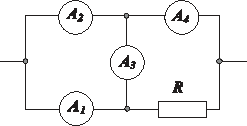
\includegraphics[width=0.6\linewidth]{2008-lahg-04-yl}
\end{center}

\hint
Mõlema kontuuri jaoks saab rakendada Ohmi või Kirchhoffi
seadusi.

\solu
Märgime skeemil voolude oletatavad suunad ning valime kontuurides $ACB$ ja $CDB$
liikumise suunaks päripäeva.

\begin{center}
	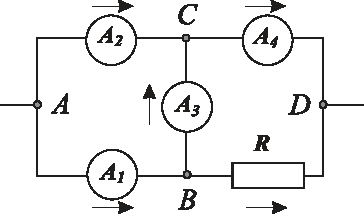
\includegraphics[width=0.6\linewidth]{2008-lahg-04-lah}
\end{center}

Kirchhoffi 2. seaduse põhjal kontuuris $ACB$
\[
I_2r - I_3r - I_1r = 0 \quad\Rightarrow\quad I_3 = I_2 - I_1 = \SI{2}{A}.
\]
Kirchhoffi 1. seaduse põhjal punktis $B$
\[
I_1 = I_3 + I_R \quad\Rightarrow\quad I_R = I_1 - I_3 = \SI{1}{A}.
\]
Kirchhoffi 1. seaduse põhjal punktis $C$
\[
I_4 = I_2 + I_3 = \SI{7}{A}.
\]
Ning lõpuks Kirchhoffi 2. seaduse põhjal kontuuris CDB
\[
I_4r - I_RR + I_3r = 0 \quad\Rightarrow\quad 9r - R = 0 \quad\Rightarrow\quad R/r = \num{9}.
\]
\probend